%! TeX Program = LuaLaTeX
\makeatletter
\def\ltj@stdyokojfm{eva/{jp,nstd}}
\makeatother
\documentclass[twoside]{ltjsarticle}
\usepackage{graphicx}
\usepackage[hiragino-pron, match, deluxe]{luatexja-preset}
\setmainfont{Linux Libertine O}
\setsansfont{Linux Biolinum O}
\setmonofont[Scale = MatchLowercase, FakeStretch = 1.137121]{Iosevka Slab}
\usepackage{luatexja-adjust}
\ltjenableadjust[priority = true]
\usepackage{listings}
\lstset{
    basicstyle = \ttfamily\small,
    breaklines = true,
    columns = fullflexible,
    keepspaces = true,
    numbers = left,
    numberstyle = \tiny,
    stepnumber = 1,
    gobble = 4,
    numbersep = 6pt,
    escapechar = §
}
\usepackage{hyperref}
\hypersetup{
    hidelinks,
    pdftitle = {Evangelion-JFM},
    pdfauthor = {黄京},
    pdfsubject = {TeX},
    pdfkeywords = {Japanese Font Metric},
    pdfstartview = FitV
}
\long\def\feature#1#2#3{{\vskip8pt\vbox{\normalsize\parindent=\zw\hangindent=2\zw\rightskip=2\zw\texttt{#1 --> ({\itshape #2\/})}\\\indent#3\par}}}
\def\meta#1{{\normalfont\rmfamily\itshape$\langle$#1\/$\rangle$}}
\def\空{\quad}
\def\段{\par}
\def\LuaTeX{Lua\kern-.2ex\TeX}
\def\pTeX{p\kern-.2ex\TeX}
\def\pdfTeX{pdf\TeX}
\title{\sffamily\bfseries Evangelion Japanese Font Metric for \LuaTeX}
\author{\large \url{https://github.com/RadioNoiseE/Evangelion-JFM}\\\url{https://www.ctan.org/pkg/evangelion-jfm}}
\date{\西暦\today\quad{}黄京}
\begin{document}
\lstset{doubleletterspace = true}
\maketitle

\begin{abstract}
    本ドキュメントは、高品質な中国語および日本語のドキュメントを組版するための日本語フォントメトリック「Evangelion Japanese Font Metric(以下「\textsf{Eva-JFM}」とする)」を紹介するものです。このメトリックは、縦書きと横書きの両方のテキストに対して、従来の中国語、簡体字中国語、および日本語のフォントとともに使用できます。これは、\LuaTeX-ja で提供される優先機能を最大限に活用するフォントメトリックを提供し、標準\cite{jlreq}に基づき、一部の高度な(すなわち、めったに使用されない)機能をサポートすることを目的としています。\段
    本ドキュメントは、完全なものではありません。文法的な(および文脈的な)エラーが多数含まれている可能性があります。
\end{abstract}

\tableofcontents

\section{背景情報と簡単な紹介}
{\TeX}は「美しい本の制作」を目的とした強力な組版システムであり、英語ベースのテキストの組版には完全に対応しています。しかし、CJテキストのサポートは限られています\footnote{おそらく普遍的に認められたCJ文字セット標準やエンコーディングシステムが存在しなかったためかもしれません。}。{\TeX}でCJテキストを扱うために、マクロ拡張(\textsf{CJK}など)やエンジン拡張が開発されました。最も影響力のあるものの1つが{\pTeX}(シリーズ)です。\段
{\pTeX}は仮想フォント方式を使用し、TrueTypeやOpenTypeフォントを\texttt{TFM/VF}ファイルを使ってマッピングします。マクロを介したフォント設定には対応せず、PDF形式の出力にも対応していません。その利点は、伝統的な日本語のタイポグラフィレイアウト要件を扱うための証明済みの能力にあります。\段
{\pdfTeX}は、PDFファイルを直接出力できる{\TeX}エンジンの拡張です(その名の通り)。ただし、Unicodeや現代のフォント形式(TrueTypeやOpenTypeベクターフォント形式)に対するサポートは限定的です。\段
{\LuaTeX}は{\pdfTeX}をベースにしています。Luaの組み込みにより、読み込みモジュールを使用してUnicodeをサポートし、\textsf{fontloader}を使用して現代のフォントをサポートすることができます。マクロベースのフォント設定機能は\textsf{luaotfload}によって提供されます。\段
\LuaTeX-jaは{\pTeX}と{\LuaTeX}の移植版と見なすことができます。{\LuaTeX}を使用する場合、マクロによるフォント設定がサポートされるため、{\pTeX}の\texttt{VF}ファイルを保持する必要はありません。しかし、一部の高度な機能(「優先度」機能や仮想的な文字など)は、いわゆるJFMファイルで残され、拡張されました。\段
このドキュメントでは、高度なJFMファイルである\textsf{Eva-JFM}を説明します。{\LuaTeX}のコールバックを使用して、\texttt{Eva-JFM.lua}にCJテキスト組版に必要な機能を埋め込みます(おそらく)。現在サポートされている機能は、「繁体字中国語」、「簡体字中国語」、「日本語」、「縦組」、「ぶら下げ」、「行間句読点」、「全角歐文」、「半角歐文」、「非標準」。\段

\section{インストールとローカル設定}
ソースファイルはGithubにホストされ、CTANにもアップロードされています。ユーザーは単純に
\begin{lstlisting}
    tlmgr install evangelion-jfm
\end{lstlisting}
(または他のパッケージマネージャーを使用することもできます)を使用してインストールできます。ただし、CTANブランチが常に更新されているわけではないことに注意してください。 開発者はまた
\begin{lstlisting}
    mkdir Evangelion-JFM [&&] cd Evangelion-JFM
    git clone https://github.com/RadioNoiseE/Evangelion-JFM
\end{lstlisting}
を使用して最新バージョンを抽出し、それを\texttt{TEXMF}ディレクトリに移動することもできます。たとえば
\begin{lstlisting}
    ~/Library/texlive/2023/texmf-dist/tex/luatex/eva-jfm
\end{lstlisting}
あなたの{\TeX}配布が\texttt{Ls-R}データベースを更新するためにを
\begin{lstlisting}
    mktexlsr
\end{lstlisting}
を必要とする場合は、それを実行してください。\段
\textsf{Eva-JFM}はほとんどの場合、ローカル設定を必要としませんが、特別な要件がある場合は、セクション\ref{sec:config}を参照してください。

\section{使用}
\begin{lstlisting}
    \usepackage{luatexja-fontspec, luatexja-adjust}
    \setmainjfont{Source Han Serif TC}[Language = Chinese Traditional, TateFeatures = {JFM = eva/{vert, trad, nstd}}]
    \ltjenableadjust[priority = true]
\end{lstlisting}
\indent 上記は、縦書きの伝統的な中国語フォントを使用して縦書きのテキストを組版する例です。注意が必要ですが、縦書きのテキストをサポートするドキュメントクラスを読み込むか、\texttt{\string\tate}コマンドを使用する必要があります。\LuaTeX-jaのJFM構文は、次のようになります
\begin{lstlisting}
    jfm = §\meta{JFM name}§/{§\meta{JFM features}§}
\end{lstlisting}
{\LaTeX}の場合、\texttt{\string\setmainjfont}を使用する場合、最も一般的なケースは、以下のようになります
\begin{lstlisting}
    \setmainjfont{§\meta{font name}§}[Language = §\meta{language name}§, §\meta{dir}§ = {JFM = §\meta{JFM name}§/{§\meta{JFM features}§}}]
\end{lstlisting}
オプションの\meta{font name}は、文書のメインフォントとして指定したいフォントの名前です。日本語のフォントを使用する場合、\meta{language name}は自動的に\LuaTeX-jaによって補完されるため、無視してください。この場合、伝統的な中国語フォントには\texttt{Chinese Traditional}、簡体字中国語フォントには\texttt{Chinese Simplified}を指定する必要があります(これを指定しないと、出力が間違った細部、例えば句読点の形状と方向が変わってしまう可能性があります)。\meta{dir}は、縦書きの場合は\texttt{TateFeatures}、横書きの場合は\texttt{YokoFeatures}に設定します。JFMの名前は\meta{JFM features}オプションで指定します\footnote{\LuaTeX-jaは\texttt{jfm-\meta{JFM name}.lua}という方法でJFMファイルを検索します。}。最後に、\meta{JFM features}キーにJFMの特徴を入力してください。これらは、セクション\ref{sec:feat}で説明されています。
上級ユーザーの場合、以下を使用することをお勧めします
\begin{lstlisting}
    \def\ltj@stdyokojfm{eva/{§\meta{JFM features}§}}
\end{lstlisting}
またはNFSSを使用することもできます。\段
他の場合でJFMを設定するには、\LuaTeX-jaのドキュメント\cite{luatexja-doc}を参照してください。

\section{サポートされる機能}
\label{sec:feat}
このセクションでは、\texttt{Eva-JFM}に組み込まれたすべての機能を概観します。それらは5つのグループに分けられ、それぞれ次の5つのサブセクションで説明されています。

\subsection{言語機能}
このセクションから1つの機能を指定する必要があります。そうしない場合、{\TeX}はエラーを出します。\段
\feature{jp}{JaPanese}{%
    日本語フォント機能。日本語フォントを使用する場合、この機能を指定する必要があります。伝統的な中国語と簡体字中国語の機能とは異なり、縦書き時に疑問符や感嘆符の後に挿入されるグルー、および句読点の位置が異なります。これは、\texttt{lgp}機能および内部グルーピングに影響します。
}
\feature{trad}{TRADitional chinese}{%
    伝統的な中国語機能。伝統的な中国語フォントを使用して組版する場合は、この機能を指定する必要があります。他の2つとの違いは、中央に配置された句読点です。そのため、それに隣接するグルー、行末の調整、および句読点間のカーニングは特別なものです。
}
\feature{smpl}{SiMPLified chinese}{%
    簡体字中国語機能。簡体字中国語フォント用です。すべての句読点は横に配置されています。したがって、その位置は注意して扱われます。\textsf{Eva-JFM}はいくつかの珍しい状況も考慮しています。なお、疑問符と感嘆符の後の空きは日本語フォント機能とは異なります。
}

\subsection{方向機能}
このセクションの機能は、すべての他の機能と互換性があります。\段
\feature{vert}{VERTical writing}{%
    縦組機能。カーニング、内部グルーピングなどに影響します。縦書き時には、これを指定する必要があります。
}

\subsection{拡張機能}
ぶら下げ\texttt{hgp}機能を除くすべての機能は、\texttt{vert}機能に依存して動作します(縦書きテキストで必要なため)。\段
\feature{extd}{EXTenDed font}{%
    拡張フォント機能。デフォルトの比率は、\textit{x\/}:\textit{y\/}=100:80で、\textit{x}は幅、\textit{y}は高さを表します。\texttt{extd=\meta{ratio}}(デフォルトの\meta{ratio}は1.25)を使用してカスタマイズできます。\texttt{extend}(\textsf{luaotfload})または\texttt{FakeStretch}(\textsf{fontspec})と。
}
\feature{lgp}{LineGap Punctuations}{%
    ラインギャップの句読点機能。これは、いくつかの句読点をラインギャップに掛けます。\texttt{jp}機能で使用すると、いくつかの違いが発生します。詳細については、セクション\ref{sec:lgp}を参照してください。
}
\feature{hgp}{HanGing Punctuations}{%
    行末に句読点を「ハング」する句読点機能をぶら下げます(少し目立つようにする)。繁体字中国語フォント結果がやや(むしろ)奇妙であるため、この機能はサポートしていません。
}

\subsection{歐文機能}
このセクションの機能を使用する前に、JAchar範囲を\texttt{\string\ltjsetparameter}で設定する必要があります。また、対応するOpenType機能と併用することが推奨されています。\段
\feature{hwid}{Half WIDth}{%
    半角英語文字機能。各アルファベットをCJ文字の幅のちょうど0.5倍の箱に配置します。これはグリフを伸ばしたり縮めたりするわけではなく、スペーシングを調整するだけであることに注意してください。したがって、OpenType機能\texttt{hwid}が設定されていない場合、英語の文字は単に重なり合います。すべてのカーニングとイタリックの補正も失われます(これは将来のバージョンで修正されるかもしれません)、\texttt{xkanjiskip}パラメータは無視されます。注意して使用してください。
}
\feature{fwid}{Full WIDth}{%
    全角英語文字機能。スペーシングが逆に広がりますが、機能\texttt{hwid}と同様です。
}

\subsection{ダーク機能}
以下の機能を使用する前に、説明を注意深く読んでください。\段
\feature{nstd}{Non STandarD}{%
    この機能は、句読点のカーニングに対する標準的な優先ルールを無視します。日本語のテキストレイアウト要件\cite{jlreq}では、ピリオドの優先度がカンマよりも高いとされているため(つまり、ピリオドは伸ばしやすい)、この機能によってカンマの優先度がピリオドよりも高くなります。\textsf{luatexja-adjust}の\texttt{priority}機能が有効になっている場合にのみ機能します(\texttt{true}に設定)。
}
\feature{plain}{PLAIN punct kerning style}{%
    句読点間隔の調整は実行しません,\texttt{verbatim}環境のために設計された。提供されたフックで使用することをお勧めします。
}

\section{行間句読点機能}
\label{sec:lgp}
ここでは、行間句読点に関する詳細な情報、発生する可能性のある問題、および解決策が提供されます。
\subsection{「垂直懸垂」とは}
垂直懸垂は、中国の古典的な書籍に見られる、句読点と伝統的な縦書き組版方法を組み合わせたものである。\段
\textsf{Eva-JFM}では、ピリオドとカンマだけが懸垂されますが、\texttt{Eva-JFM}ではコロンとセミコロンの向きのため、これらの文字は懸垂できません。日本語フォントにはこの点に関して異なる特徴があります。\段
これらの文字は、グリフの下右に懸垂されます。詳細については次のサブセクションを参照してください。

\subsection{懸垂位置}
\begin{figure}[htb]
    \centering
    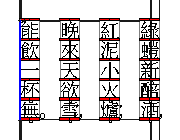
\includegraphics[height = 12\zh]{figure/fig-tc.pdf}\空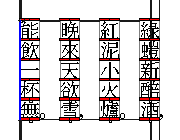
\includegraphics[height = 12\zh]{figure/fig-jp.pdf}
    \caption{垂直懸垂の機能}
    \label{fig:lgp}
\end{figure}
図\ref{fig:lgp}~に示すように、これらの懸垂句読点の位置は、以下のルールに従って決定されます。カスタマイズについては、サブセクション\ref{sec:config}を参照してください。ルールの優先順位は早い順に高くなります。
\begin{itemize}
    \item 3つのフォントのスタイルは統一されています;
    \item 異なる句読点における同じ要素の位置は同じであるべきです;
    \item 句読点のグリフは漢字の境界に接触するべきです;
    \item 異なる句読点の位置は、それぞれのグリフの形状、サイズ、デザインに応じて異なる場合があります。
\end{itemize}

\subsection{ユーザー設定}
\label{sec:config}
この機能はSource Hanフォントシリーズ(思源系列)に設計されています。異なるフォントによって異なる句読点があるため、出力が誤った結果になる可能性があります(オーバーラップ、揃っていないなど)。そのため、懸垂句読点の位置をカスタマイズするための2つの方法が提供されています。

\subsubsection{パラメータの変更}
\texttt{Eva-JFM}では、これらの懸垂句読点の位置に関するパラメータを含むテーブルは以下のようになります
\begin{lstlisting}
    [101,2] ==> [1]; [201,2] ==> [2]; [301,2] ==> [3].
\end{lstlisting}
上下のパラメータを調整して、出力を修正してください。
また、最後のセクション『実装』も参照してください。

\subsubsection{追加フォントの使用}
句読点のグリフを抽出して、新しいフォントにパッケージ化し、後で行頭の句読点に使用することが、2番目の解決策です(\textit{Fontforge\/}などのプログラムを使用できます)。また、句読点だけのために別のフォントをロードすることもできますが、CJフォントを{\TeX}のメモリにロードするコストは高くなります。\段
このフォントをインストールした後、\LuaTeX-jaで提供される\texttt{AltFont}キーを使用して、句読点を置き換えることができます。実際のコードは上記に示されています:
\begin{lstlisting}
    \setmainjfont[
        Language = §\meta{language}§,
        TateFeatures = {
            JFM = eva/{vert, lgp, §\meta{language}§},
            AltFont = {
                {Range = "§\meta{utf-8 code}§, Font = §\meta{symbol font}§}
            }
        }
    ]{§\meta{main font}§}
\end{lstlisting}
最初の\meta{language}オプションには、日本語、繁体字中国語、簡体字中国語のいずれかを入力し、もう一方は対応するJFMの機能のためのものです。 \meta{utf-8 code}は、置き換えたい句読点を「句読点フォント」で選択します\footnote{Unicodeのコードポイントは\url{https://www.unicode.org/charts/unihanrsindex.html}で確認できます。}。最後に、\meta{symbol font}と\meta{main font}オプションは、「句読点フォント」とメインフォントのためのものであることが明らかです。\段
開発者は、以下のように NFSS を使用することを推奨します
\begin{lstlisting}
    \DeclareAlternateKanjiFont{§\meta{base encoding}§}{§\meta{base family}§}{§\meta{base series}§}{§\meta{base shape}§}{§\meta{alt encoding}§}{§\meta{alt family}§}{§\meta{alt series}§}{§\meta{alt shape}§}{§\meta{range}§}
\end{lstlisting}
オプション\meta{base}と\meta{alt}は、メインフォントと「句読点フォント」のためのものです。\段
詳しい構文や使用方法、例については、\LuaTeX-jaのドキュメント\cite{luatexja-doc}を参照してください。

\section{インスピレーション}
\textsf{Eva-JFM}の内部グループ化は、\texttt{min10.tfm}~\cite{min10}に触発されています。また、優先度の特徴のデータは、阿部紀行氏の\texttt{jlreq.lua}~\cite{ltxjlreq}から一部引用しています。\段
このJFMの名前は、庵野秀明氏のアニメーション『新世紀エヴァンゲリオン』。

\begin{thebibliography}{9}
    \addcontentsline{toc}{section}{\refname}
    \bibitem{jlreq} W3C Japanese Layout Task Force~(ed). \newblock Requirements for Japanese Text Layout (W3C Working Group Note), 2022, 2023. \newblock \url{https://www.w3.org/TR/jlreq/}.
    \bibitem{luatexja-doc} \LuaTeX-jaプロジェクトチーム. \newblock \LuaTeX-jaパッケージ, 2022, 2023.
    \bibitem{unicode} The Unicode Consortium. \newblock The Unicode Standard Version 15.0 - Core Specification, 2022.
    \bibitem{tex-by-topic} Victor Eijkhout. \newblock \TeX{} by Topic, A \TeX nician's Reference, Addison-Wesley, 1992.
    \bibitem{min10} 乙部厳己. \newblock min10フォントについて. \newblock \url{http://argent.shinshu-u.ac.jp/~otobe/tex/files/min10.pdf}.
    \bibitem{ltxjlreq} 阿部紀行. \newblock Jlreq Document Class, 2022. \newblock \url{https://github.com/abenori/jlreq}.
    \bibitem{evang} 庵野秀明. \newblock 新世紀エヴァンゲリオン.
\end{thebibliography}


\end{document}
